% Include the header of the document.
\documentclass[a4paper]{article}

% TeX Packages.
\usepackage[T1]{fontenc}              % Use 8-bit T1 fonts
\usepackage[backend=bibtex]{biblatex} % Citing
\usepackage[english]{babel}           % Set English as main language
\usepackage[intoc, english]{nomencl}  % Nomenclature
\usepackage[utf8]{inputenc}           % Allow utf-8 input
\usepackage{algorithmicx}
\usepackage{algorithm}
\usepackage{algpseudocode}
\usepackage{amsfonts}
\usepackage{amsfonts}                 % Blackboard math symbols
\usepackage{amsmath}                  % AMS Math
\usepackage{amssymb}                  % AMS Symbols
\usepackage{amsxtra}
\usepackage{appendix}                 % Appendix
\usepackage{array,epsfig}
\usepackage{booktabs}                 % Professional-quality tables
\usepackage{caption}                  % Captions
\usepackage{color}
\usepackage{csquotes}                 % Context sensitive quotation facilities
\usepackage{float}                    % Float control
\usepackage[top=20mm,
  bottom=20mm,
  left=20mm,
  right=20mm]{geometry}                 % Easily define margins
\usepackage{graphicx}                 % Graphic materials (e.g., images)
\usepackage{hyperref}                 % Hyperlinks
\usepackage{listings}
\usepackage{microtype}                % Microtypography
\usepackage{ntheorem}
\usepackage{rotating}                 % Allow page rotation (e.g., for large table)
\usepackage{subcaption}               % Subcaptions and subfigures.
\usepackage{tikz}                     % Drawings
\usepackage{url}                      % Simple URL typesetting

\date{\today}
\author{Joeri Hermans \\ \href{mailto:joeri.hermans@doct.ulg.ac.be}{joeri.hermans@doct.ulg.ac.be}}

\begin{document}


\title{Sloan Digital Sky Survey Analysis and Data Engineering}
\maketitle

\section{Introduction}
\label{sec:introduction}

The Sloan Digital Sky Survey\footnote{\href{https://www.sdss.org}{https://www.sdss.org}} or SDSS, is a major multi-spectral imaging and spectroscopic redshift survey using a dedicated 2.5 meter wide-angle optical telescope at Apache Point Observatory in New Mexico, United States. The Sloan Digital Sky Survey has created the most detailed three-dimensional maps of the Universe ever made, with deep multi-color images of one third of the sky, and spectra for more than three million astronomical objects. The SDSS began regular survey operations in 2000, after a decade of design and construction.  It has progressed through several phases, SDSS-I (2000-2005), SDSS-II (2005-2008), SDSS-III (2008-2014), and SDSS-IV (2014-).  Each of these phases has involved multiple surveys with interlocking science goals.  The three surveys that comprise SDSS-IV are eBOSS, APOGEE-2, and MaNGA.\\

In this project, you will be working with data from the eBOSS (Extended Baryon Oscillation Spectroscopic Survey) experiment. eBOSS precisely measures the expansion history of the Universe throughout eighty percent of cosmic history, back to when the Universe was less than three billion years old, and improve constraints on the nature of dark energy. “Dark energy” refers to the observed phenomenon that the expansion of the Universe is currently accelerating, which is one of the most mysterious experimental results in modern physics.

\begin{figure}[H]
  \centering
  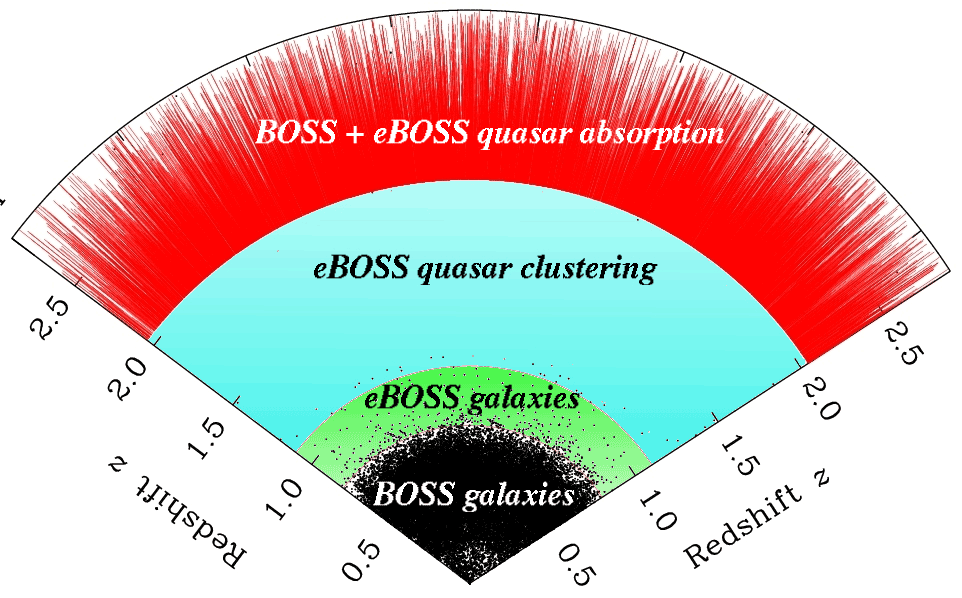
\includegraphics[width=.5\textwidth]{figures/eboss_coverage}
  \caption{Converage of the eBOSS experiment up to redshift ($z$) = 3.}
  \label{fig:eboss_coverage}
\end{figure}

In physical terms, redshift, described in Equation~\ref{eq:redshift}, happens when light or other electromagnetic radiation from an object is increased in wavelength, or shifted to the red end of the spectrum. In general, whether or not the radiation is within the visible spectrum, "redder" means an increase in wavelength – equivalent to a lower frequency and a lower photon energy, in accordance with, respectively, the wave and quantum theories of light. Some redshifts are an example of the Doppler effect, familiar in the change of apparent pitches of sirens and frequency of the sound waves emitted by speeding vehicles. A redshift occurs whenever a light source moves away from an observer.

\begin{equation}
  z = \Bigg(\frac{\lambda_\text{observed}}{\lambda_\text{rest}}\Bigg) - 1
  \label{eq:redshift}
\end{equation}

In astronomy, redshift can be utilized to measure the \emph{accelerating} expansion of the universe. This is exactly one of the key questions posed by the eBOSS survey. In princple, eBOSS measures this by identifying the wavelengths of emission and absorption lines, and then comparing with the known spectra in a vacuum for those elements and thereby obtaining an average redshift for all spectra using Equation~\ref{eq:redshift}.

\begin{figure}[H]
  \centering
\end{figure}

Furthermore, these emmision lines and their accompanying fluxes (number of photons that caused a certain amount of electrons to move) can be utilized whether the observed instance is a \emph{star} (subclasses of the spectral types can also be identified\footnote{\href{https://en.wikipedia.org/wiki/Stellar\_classification\#Spectral\_types}{en.wikipedia.org/wiki/Stellar\_classification\#Spectral\_types}}), \emph{galaxy} or a \emph{quasar}, as shown in Figure~\ref{fig:spectra_galaxy} and Figure~\ref{fig:spectra_star}.

\begin{figure}[H]
  \centering
    \begin{minipage}[b]{0.48\textwidth}
    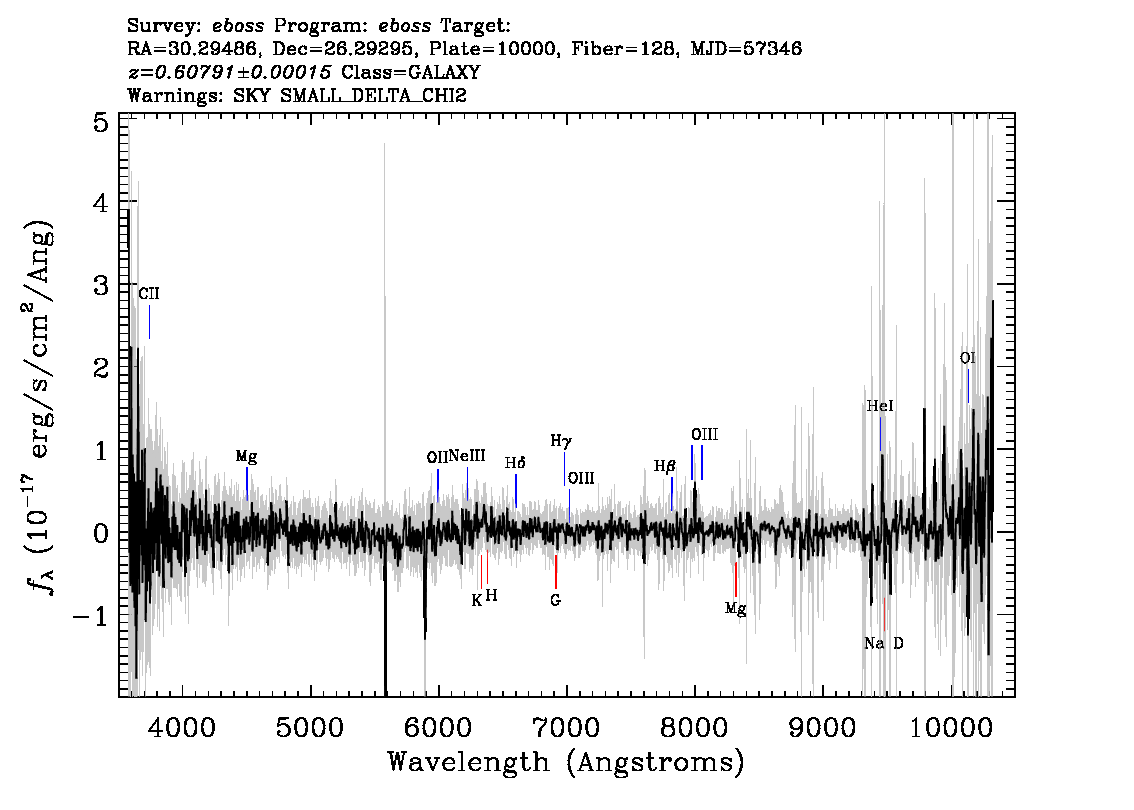
\includegraphics[width=\textwidth]{figures/spectra_galaxy_1}
    \caption{Spectra with accompanying fluxes of a galaxy with identified absorption lines.}
    \label{fig:spectra_galaxy}
  \end{minipage}
  \hfill
  \begin{minipage}[b]{0.48\textwidth}
    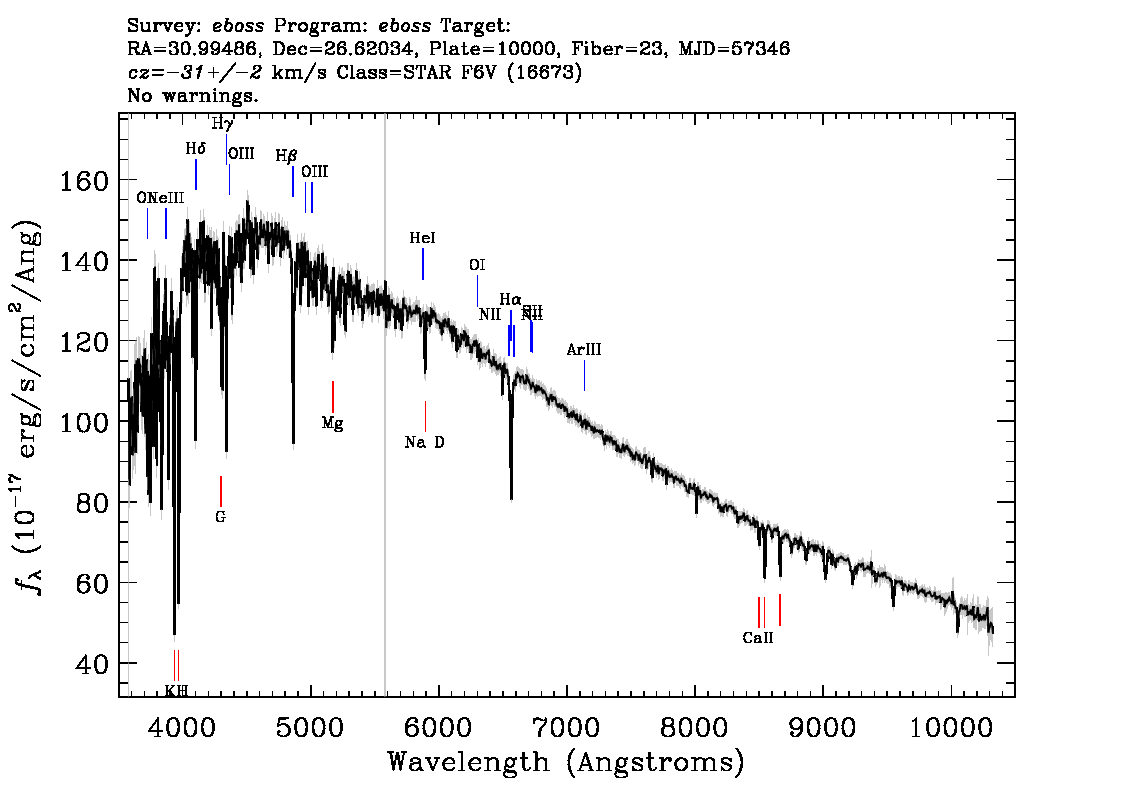
\includegraphics[width=\textwidth]{figures/spectra_star_1}
    \caption{Spectra with accompanying of a star with identified absorption lines.}
    \label{fig:spectra_star}
  \end{minipage}
\end{figure}

\begin{figure}[H]
  \centering
  \begin{minipage}[b]{.4\textwidth}
    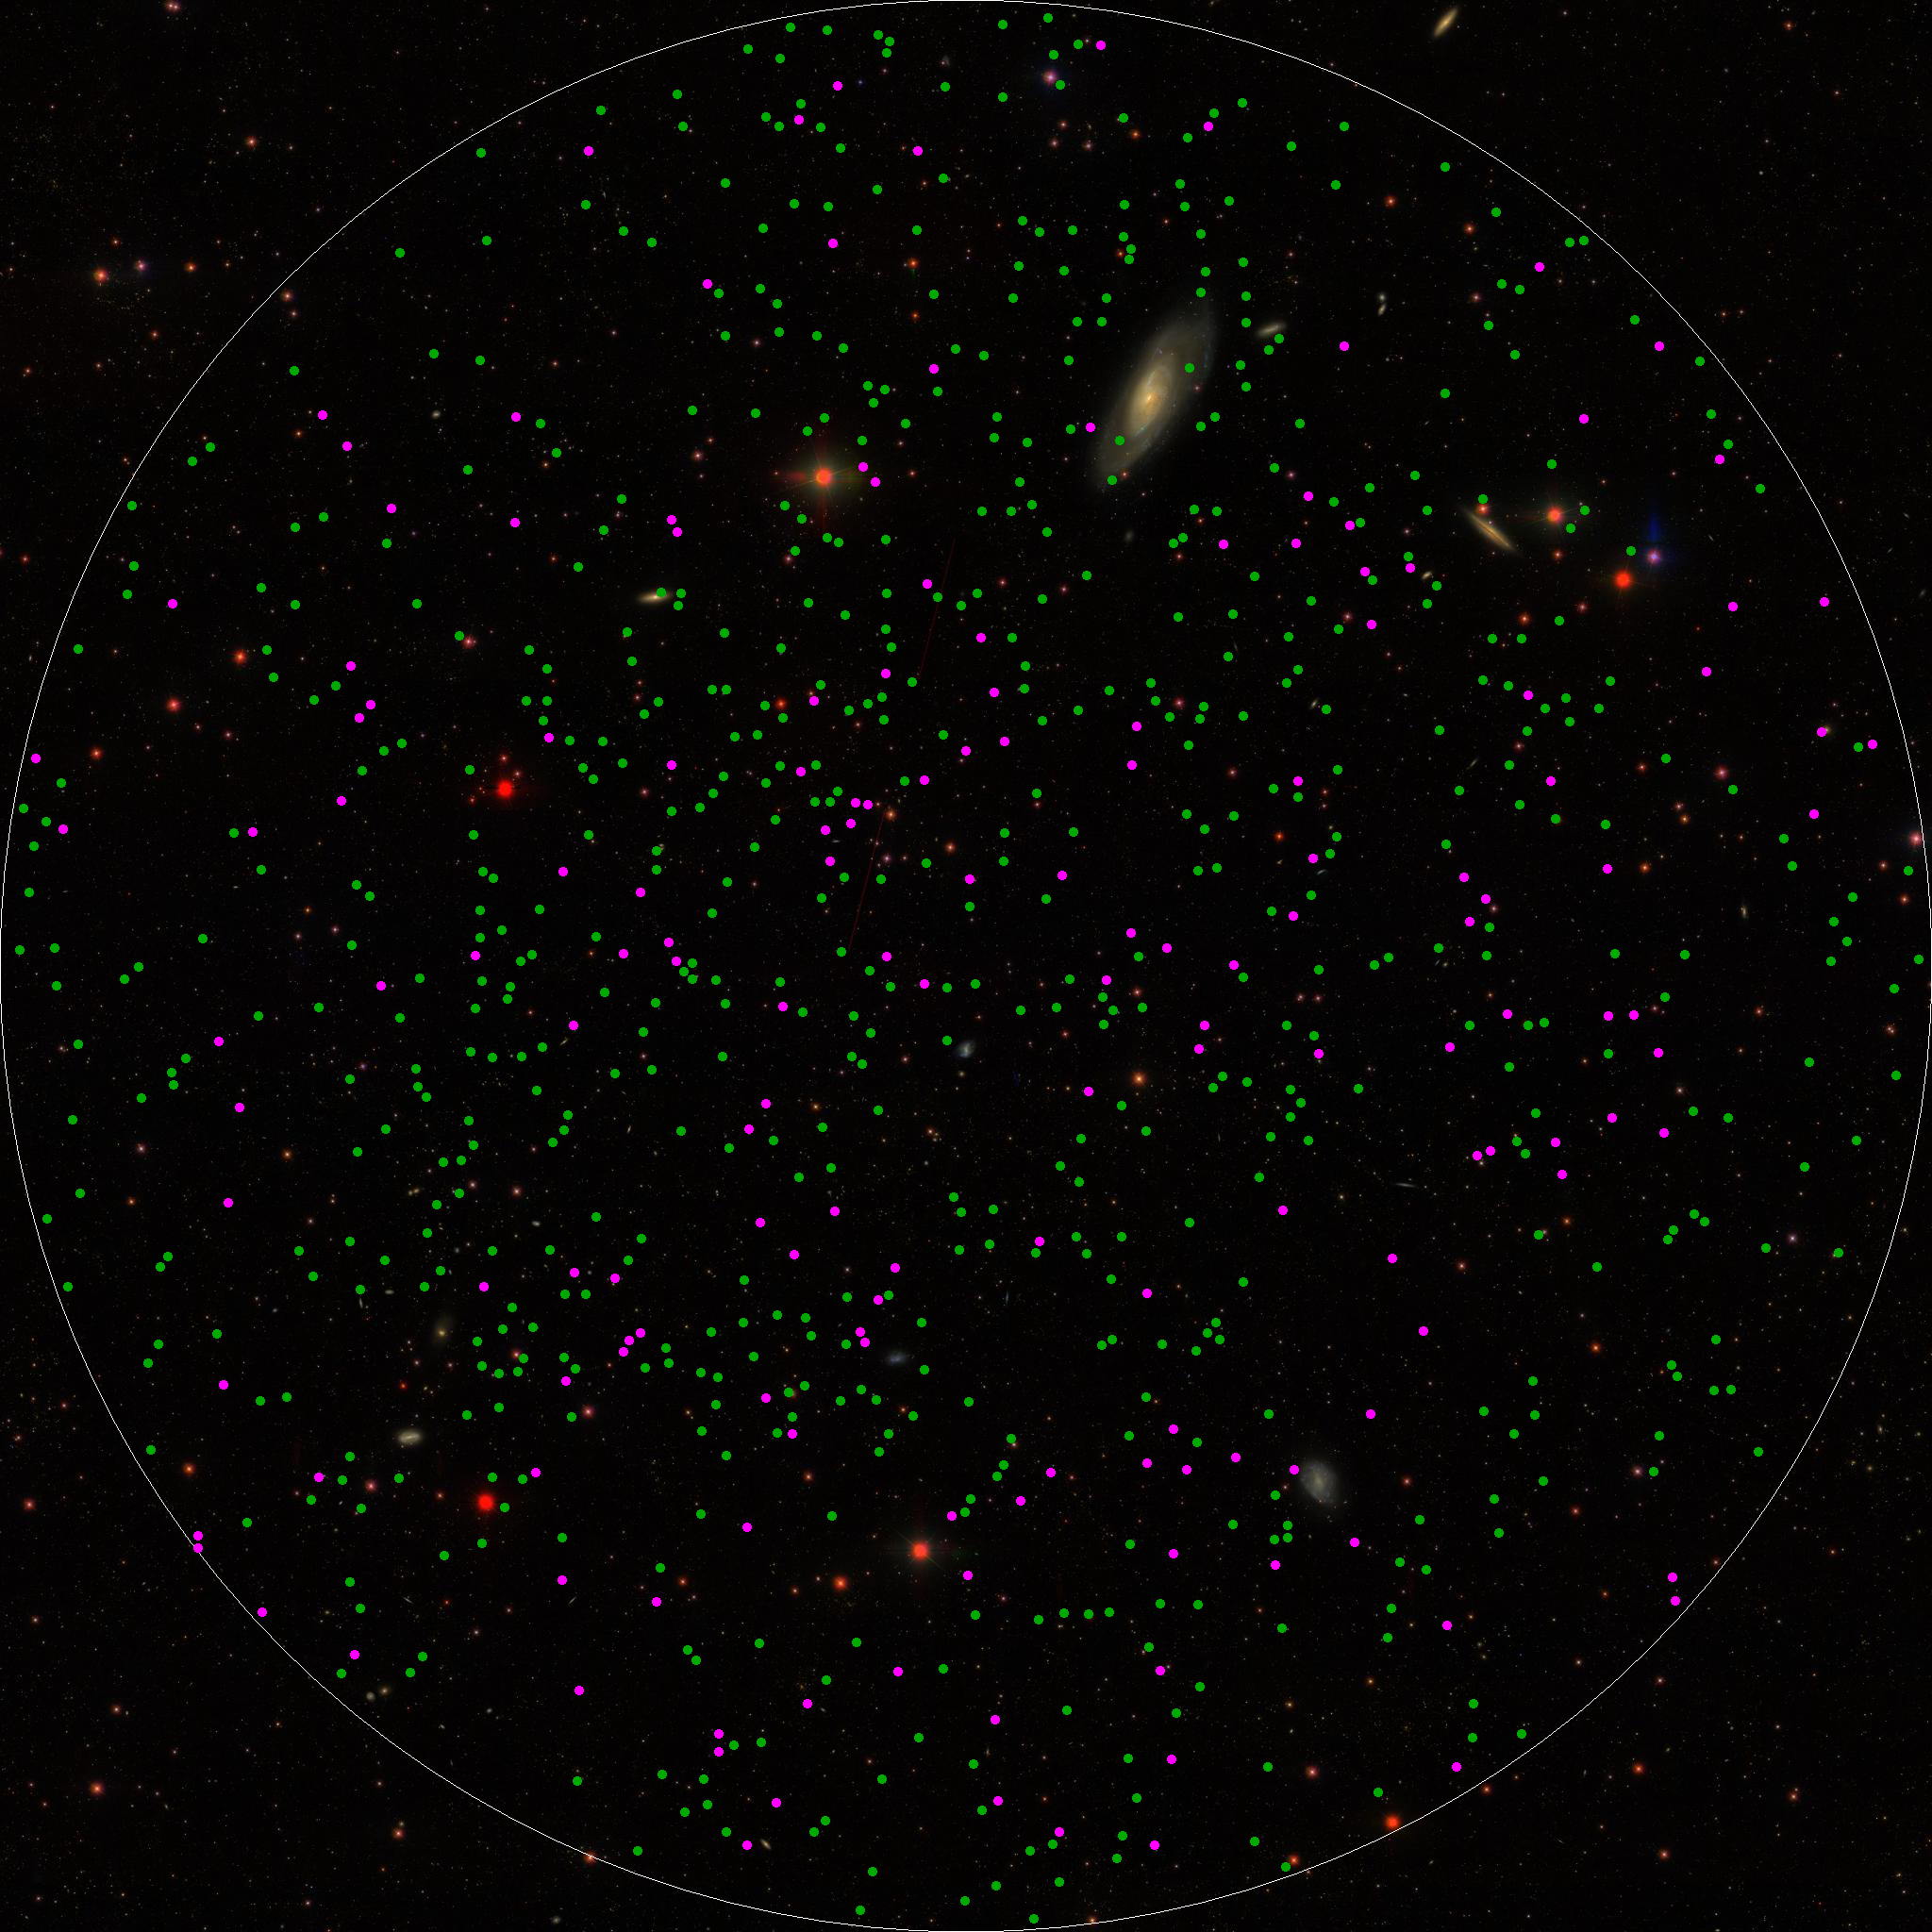
\includegraphics[width=\textwidth]{figures/plate}
    \caption{SDSS plate and target selection (green for galaxies and purple for quasars).}
    \label{fig:sdss_plate}
  \end{minipage}
  \hfill
  \begin{minipage}[b]{.45\textwidth}
    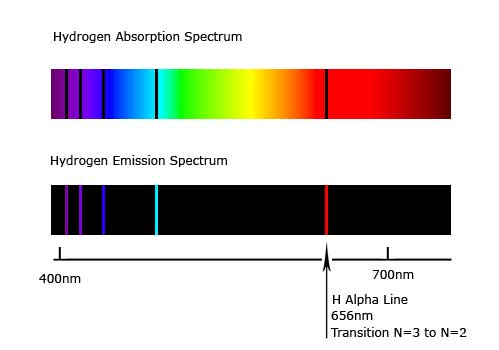
\includegraphics[width=\textwidth]{figures/hydrogen-spectra}
    \caption{Balmer Series of the Hydrogen. Shows absorption and emission lines from orbital 2 to 3 and higher.}
    \label{fig:balmer_series}
  \end{minipage}
\end{figure}

The data collection procedure is done by drilling several holes in an aluminimum plate which are positioned in a particular way to obtain individual fluxes of target objects, as shown in Figure~\ref{fig:sdss_plate}. This approach allows the eBOSS survey to observe multiple targets at once by attaching an optical \emph{fiber} to every drilled hole, causing the individual observations to be independent of each other. Furthermore, this approach allows SDSS to filter out nearby galaxies which are known to be \emph{blueshifted} (negative redshift, i.e., objects which are blueshifted have a component which move towards us), and obtain the individual background flux for every observed object.

\newpage
\section{Data Products}
\label{sec:data_products}

The data of the eBOSS survey that I will provide you with is only a partial subset of the complete eBOSS survey data. For every plate and MJD (Modified Julian Data), SDSS provides several processed data products:

\begin{itemize}
  \item A collection of \emph{spZall} data files.
  \item A collection of \emph{spZbest} data files.
  \item A collection of \emph{spZline} data files.
  \item A single \emph{platelist} file describes all plates and their data quality.
\end{itemize}

The most relevant data product to this project, \emph{spZall}, contains the summary statistics of all fibers on a single plate, including the class and subclass of the object that is being observed. The remaining data files, \emph{spZbest} and \emph{spZline}, hold the data on the best fits of the observed data, and data on the fluxes of the received wavelengths respectively. All data in stored in the FITS format, which is a common format in astronomy. Intuitively, the format can be described as a collection of tables, and images. For instance, you could produce a FITS file which stores an image of the object you are observing, and also a table which describes every wavelength of the light that has been received.

\section{Deliverables \& Logistics}
\label{sec:deliverables}

To complete this project succesfully, I would like you to solve and provide proof for the following questions. These questions have to be solved with Apache Spark. The proof for these questions have to be provided in a \emph{reproducable} Jupyter Notebook with a full description what you are doing (using Markdown cells). This will suffice as your report. The project has to executed in groups with a maximum number of two persons per group. Groups need to be registered on the submission site of Montefiore. The deadline of this project is 22 December 2017 at midnight.

\begin{enumerate}
  \item \emph{Looking at galaxies, is the expansion of the Universe uniform across all regions of the sky? Meaning, is the redshift of the galaxies about equal across the sky?}
  \item \emph{Is the expansion of the Universe accelerating?}
  \item \emph{What is the average velocity of the galaxies which are redshifted?}
  \item \emph{What is the average velocity of the quasars which are redshifted?}
  \item \emph{Are there galaxies with a relatively small flux which are blueshifted?}.
  \item \emph{What is the distribution of the spectral type of all observed stars?}
\end{enumerate}

To solve these questions, you will be reading and parsing the data products described in Section~\ref{sec:data_products}. However, in order to do this in an efficient manner, you most likely have to come up with an intermediate representation constructed from the original data products to perform efficient IO, i.e., it does not really make sense that you have to parse the original data structure every time when you wish to extract some valuable information. Before obtaining such a representation, you also have to figure out a way to efficiently parse the original data products (in FITS). To summarize, you need to provide \emph{code to transform the original data into some other representation} in a way that it efficiently can be read into an Spark RDD or a Spark DataFrame.\\

Finally, to improve the SDSS query engine, I would like you to come up with a method which is able to efficiently generate plots such as in Figure~\ref{fig:spectra_galaxy}, and Figure~\ref{fig:spectra_star}, for a specific region of the sky, i.e., given a specific range of \emph{right ascension} and \emph{declination}. This method will be utilized to evaluate the efficiency of your data representation (so optimize your schema for these type of queries).

\section{Bonus}
\label{sec:bonus}

A bonus point (1/20) is awarded to the group which is able to provide the fastest average random query time over the complete eBOSS dataset (171 GB). The query that will be ran to evaluate the performance of your data architecture, will be concerned with selecting objects in a particular section in the sky. Meaning given a minimum RADEC (Right Ascenssion and Declination), and a maximum RADEC, return the list of objects which are within this coordinate system. Your result might have practical implications as well, since the current SDSS query tool is \emph{very} slow.

\section{Cluster Access}
\label{sec:cluster_access}

For this project, you will be able to deploy your code on a multi-node Spark cluster. The connection details, and examples of how to submit a job to the cluster, will be released in the following days in this document. An e-mail will be sent the cluster configuration has been finalized.

\section{Assistance}
\label{sec:assistance}

After every lecture, the assistent will be present to help you with questions surrounding this project.

\section{Data Access}
\label{sec:data_access}

To prevent you from downloading all the required SDSS data, a stick will be available at the start and end of every lecture session. This USB stick contains only a specific subset of the complete eBOSS survey dataset. However, it can be used to provide proof for the questions posed above.

% Include the footer of the document.
\end{document}

